% math.tex — \input'd from thesis/experiments.tex
%
% Random sweep of systolic ratios on random 4D polytopes.
%
% Sources:
%   - Generated data: experiments/random-sweep/random-sweep.jsonl
%   - Plot script: experiments/random-sweep/analyze.py
%   - Logbook: experiments/random-sweep/logbook.md
%
% Structure:
%   - Sampling setup
%   - Summary plot and interpretation

\subsection{Random Sweep: Systolic Ratio vs Facet Count}
\label{sec:random-sweep}

We sample random 4D polytopes with facet counts $F = 5,\dots,12$ and compute
$c_{\mathrm{EHZ}}$ using the HK2017 pruned algorithm. Facet normals are sampled
uniformly on $S^3$, heights are uniform in $[0.8, 1.2]$, and polytopes are
accepted by the standard rejection sampler. The sample plan is:
$10$~polytopes for each $F=5,\dots,10$, and $5$~polytopes each for $F=11,12$.

Figure~\ref{fig:random-sweep-sys} summarizes the systolic ratio
$\mathrm{sys} = c_{\mathrm{EHZ}}^2/(2\,\mathrm{vol})$ as a function of $F$.
Each facet count shows the individual samples (scatter) and the median with
one standard deviation error bars.

\begin{figure}[h]
\centering
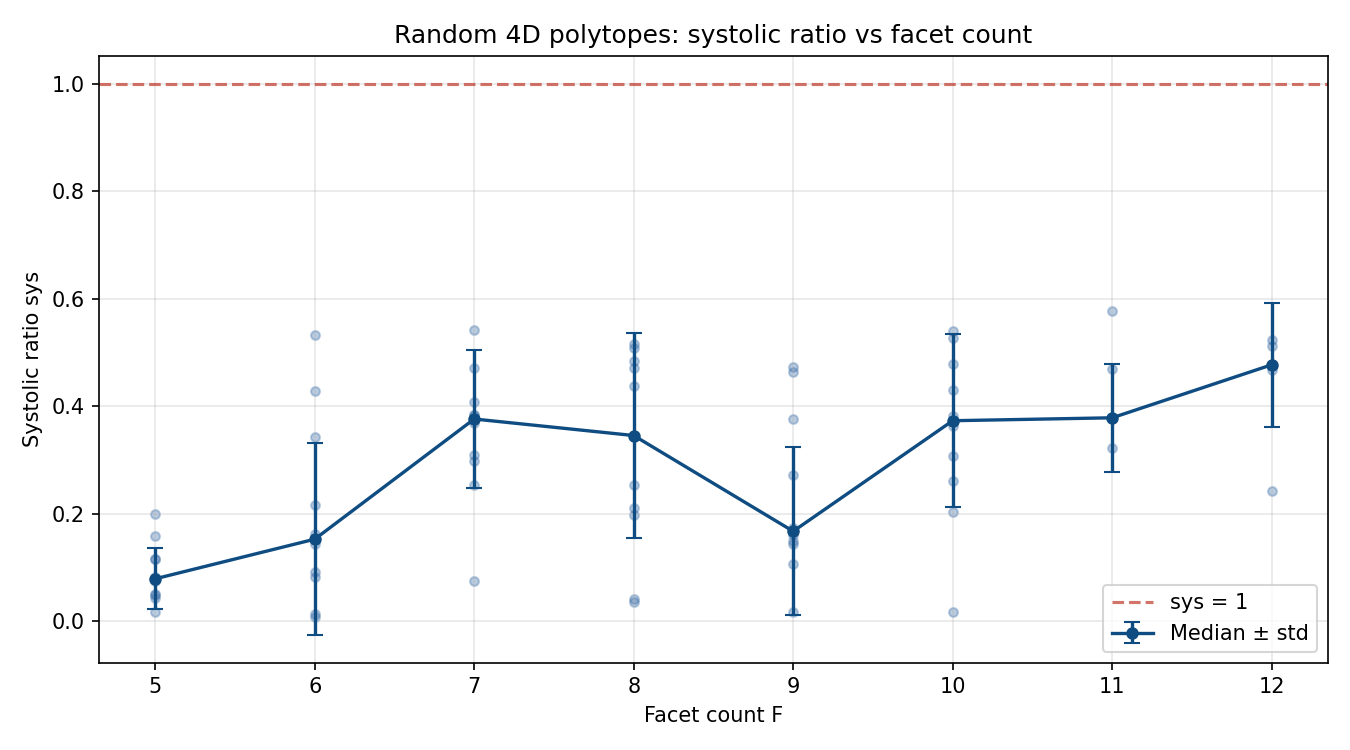
\includegraphics[width=0.9\textwidth]{../experiments/random-sweep/random_sweep_sys_vs_f.png}
\caption{Random 4D polytopes: systolic ratio vs facet count. Points show
  individual samples, and the markers with error bars show the median and
  one standard deviation for each $F$. The dashed line marks $\mathrm{sys}=1$.}
\label{fig:random-sweep-sys}
\end{figure}

\subsubsection*{Observations}

All 70 sampled polytopes satisfy~$\mathrm{sys} < 0.58$, well below the
Viterbo threshold~$\mathrm{sys} = 1$.
The median systolic ratio shows an upward trend from~$0.08$ ($F = 5$)
to~$0.48$ ($F = 12$) (Spearman $\rho = 0.47$), but the within-$F$
variance is large: at each facet count, the spread from minimum to
maximum is comparable to the median itself, and the median is
non-monotone between adjacent~$F$ values.
This suggests that polytope geometry (normal directions, height ratios)
matters as much as facet count for determining~$\mathrm{sys}$.

For comparison, the only known counterexample ($\mathrm{sys} \approx
1.047$, \cite{HaimKislevOstrover2024}) is a Lagrangian product of two
pentagons at a specific relative rotation angle.
Random generic polytopes, which have no product structure, appear to
stay far from the violation regime.
